\documentclass[journal,12pt,twocolumn]{IEEEtran}

\usepackage{setspace}
\usepackage{gensymb}
\singlespacing
\usepackage[cmex10]{amsmath}

\usepackage{amsthm}

\usepackage{mathrsfs}
\usepackage{txfonts}
\usepackage{stfloats}
\usepackage{bm}
\usepackage{cite}
\usepackage{cases}
\usepackage{subfig}

\usepackage{longtable}
\usepackage{multirow}

\usepackage{enumitem}
\usepackage{mathtools}
\usepackage{steinmetz}
\usepackage{tikz}
\usepackage{circuitikz}
\usepackage{verbatim}
\usepackage{tfrupee}
\usepackage[breaklinks=true]{hyperref}
\usepackage{graphicx}
\usepackage{tkz-euclide}

\usetikzlibrary{calc,math}
\usepackage{listings}
    \usepackage{color}                                            %%
    \usepackage{array}                                            %%
    \usepackage{longtable}                                        %%
    \usepackage{calc}                                             %%
    \usepackage{multirow}                                         %%
    \usepackage{hhline}                                           %%
    \usepackage{ifthen}                                           %%
    \usepackage{lscape}     
\usepackage{multicol}
\usepackage{chngcntr}

\DeclareMathOperator*{\Res}{Res}

\renewcommand\thesection{\arabic{section}}
\renewcommand\thesubsection{\thesection.\arabic{subsection}}
\renewcommand\thesubsubsection{\thesubsection.\arabic{subsubsection}}

\renewcommand\thesectiondis{\arabic{section}}
\renewcommand\thesubsectiondis{\thesectiondis.\arabic{subsection}}
\renewcommand\thesubsubsectiondis{\thesubsectiondis.\arabic{subsubsection}}


\hyphenation{op-tical net-works semi-conduc-tor}
\def\inputGnumericTable{}                                 %%

\lstset{
%language=C,
frame=single, 
breaklines=true,
columns=fullflexible
}
\begin{document}

\newcommand{\BEQA}{\begin{eqnarray}}
\newcommand{\EEQA}{\end{eqnarray}}
\newcommand{\define}{\stackrel{\triangle}{=}}
\bibliographystyle{IEEEtran}
\raggedbottom
\setlength{\parindent}{0pt}
\providecommand{\mbf}{\mathbf}
\providecommand{\pr}[1]{\ensuremath{\Pr\left(#1\right)}}
\providecommand{\qfunc}[1]{\ensuremath{Q\left(#1\right)}}
\providecommand{\sbrak}[1]{\ensuremath{{}\left[#1\right]}}
\providecommand{\lsbrak}[1]{\ensuremath{{}\left[#1\right.}}
\providecommand{\rsbrak}[1]{\ensuremath{{}\left.#1\right]}}
\providecommand{\brak}[1]{\ensuremath{\left(#1\right)}}
\providecommand{\lbrak}[1]{\ensuremath{\left(#1\right.}}
\providecommand{\rbrak}[1]{\ensuremath{\left.#1\right)}}
\providecommand{\cbrak}[1]{\ensuremath{\left\{#1\right\}}}
\providecommand{\lcbrak}[1]{\ensuremath{\left\{#1\right.}}
\providecommand{\rcbrak}[1]{\ensuremath{\left.#1\right\}}}
\theoremstyle{remark}
\newtheorem{rem}{Remark}
\newcommand{\sgn}{\mathop{\mathrm{sgn}}}
\providecommand{\abs}[1]{\vert#1\vert}
\providecommand{\res}[1]{\Res\displaylimits_{#1}} 
\providecommand{\norm}[1]{\lVert#1\rVert}
%\providecommand{\norm}[1]{\lVert#1\rVert}
\providecommand{\mtx}[1]{\mathbf{#1}}
\providecommand{\mean}[1]{E[ #1 ]}
\providecommand{\fourier}{\overset{\mathcal{F}}{ \rightleftharpoons}}
%\providecommand{\hilbert}{\overset{\mathcal{H}}{ \rightleftharpoons}}
\providecommand{\system}{\overset{\mathcal{H}}{ \longleftrightarrow}}
	%\newcommand{\solution}[2]{\textbf{Solution:}{#1}}
\newcommand{\solution}{\noindent \textbf{Solution: }}
\newcommand{\cosec}{\,\text{cosec}\,}
\providecommand{\dec}[2]{\ensuremath{\overset{#1}{\underset{#2}{\gtrless}}}}
\newcommand{\myvec}[1]{\ensuremath{\begin{pmatrix}#1\end{pmatrix}}}
\newcommand{\mydet}[1]{\ensuremath{\begin{vmatrix}#1\end{vmatrix}}}
\numberwithin{equation}{subsection}
\makeatletter
\@addtoreset{figure}{problem}
\makeatother
\let\StandardTheFigure\thefigure
\let\vec\mathbf
\renewcommand{\thefigure}{\theproblem}
\def\putbox#1#2#3{\makebox[0in][l]{\makebox[#1][l]{}\raisebox{\baselineskip}[0in][0in]{\raisebox{#2}[0in][0in]{#3}}}}
     \def\rightbox#1{\makebox[0in][r]{#1}}
     \def\centbox#1{\makebox[0in]{#1}}
     \def\topbox#1{\raisebox{-\baselineskip}[0in][0in]{#1}}
     \def\midbox#1{\raisebox{-0.5\baselineskip}[0in][0in]{#1}}
\vspace{3cm}
\title{Assignment-3}
\author{S. Rithvik Reddy - cs20btech11049}
\maketitle
\newpage
\bigskip
\renewcommand{\thefigure}{\theenumi}
\renewcommand{\thetable}{\theenumi}
Download all python codes from 
\begin{lstlisting}
https://github.com/rithvikreddy6300/Assignment-4/tree/main/codes
\end{lstlisting}
%
and latex-tikz codes from 
%
\begin{lstlisting}
https://github.com/rithvikreddy6300/Assignment-4/blob/main/Assignment-4.tex
\end{lstlisting}
\section*{Problem-(GATE 2011 (CS) Q-3)}
If two fair coins are flipped and atleast one of the outcomes is known to be a head, what is the probability that both outcomes are heads ?

\vspace{0.5 cm}

(A) $\dfrac{1}{3}$ \hspace{0.5 cm} (B) $\dfrac{1}{4}$ \hspace{0.5 cm} (C) $\dfrac{1}{2}$ \hspace{0.5 cm} (D) $\dfrac{2}{3}$

\section*{Solution}

Let $X=\{0,1\}$ be the set of random variables where 0 represents \textbf{Tail}, 1 represent \textbf{Head}, $x_1,x_2$ represent the outcomes of coins 1 and 2.
\begin{align}
& \pr{X=n}= \begin{cases}
\frac{1}{2} & \text{ if } n=0\\
\frac{1}{2}  & \text{ if } n=1
\end{cases}
\end{align}

Let P denote the probability that both outcomes are heads given atleast one is a head,
\begin{align}
\implies & P=\pr{x_1x_2=1|x_1\text{ or }x_2=1}\\
\implies & P=\dfrac{\pr{(x_1x_2=1)\cap (x_1\text{ or }x_2=1)}}{\pr{x_1\text{ or }x_2=1}}\\
\implies & P=\dfrac{\pr{x_1x_2=1}}{\pr{x_1\text{ or }x_2=1}}\\
\implies & P=\dfrac{\pr{x_1x_2=1}}{\pr{x_1=1}+\pr{x_2=1}-\pr{x_1x_2=1}}
\end{align}
Since $x_1$ and $x_2$ are independent events we can write
\begin{align}
 \pr{x_1x_2=1}&=\pr{x_1=1}\pr{x_2=1}\\
\implies P&= \dfrac{\frac{1}{2}\times \frac{1}{2}}{\frac{1}{2}+\frac{1}{2}-\frac{1}{2}\times \frac{1}{2}}\\
\implies P&=\dfrac{1}{3}
\end{align}
Therefore the probability of both outcomes are heads given atleast one outcome is head is $P=\dfrac{1}{3}$ option (\textbf{A}).

The probability obtained by simulation versus the calculated prob is as shown in Fig(\ref{fig_0}).
\begin{figure}[h]
    \centering
    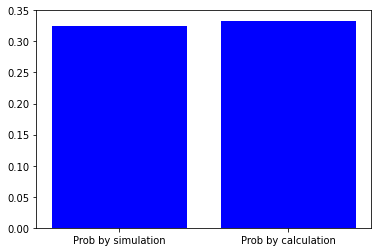
\includegraphics[width=0.4\textwidth]{img-1}
    \caption{Sim Vs Cal}
    \label{fig_0}
\end{figure}

\end{document}
